\TChapter{Análisis y diseño}{delta}
\ \\\\
En este capítulo se describe el análisis y el diseño del sistema web para el trabajo terminal propuesto, mostrando los módulos con los cual cuenta. Hasta este punto se presentan los requisitos que deberá cumplir el sistema así como los casos de uso y diagramas de secuencia.

\section{Actores y roles}
Usuario: Cualquier persona que ingrese al sistema y esté interesada en consultar noticias.


%------------------------Requisitos Funcionales ------------------%
\section[Requisitos f.]{Requisitos funcionales}

%----------------------------RF1------------------------------%
   \Dline{RF1}{Recolectar noticias}
    \begin{itemize}
      \item \textbf{Descripción:} El sistema debe recolectar noticias de forma automática de los sitios web definidos.\\
    \end{itemize}
%----------------------------RF2------------------------------%
   \Dline{RF2}{Clasificar noticias}
    \begin{itemize}
      \item \textbf{Descripción:} El sistema debe clasificar las noticias recolectadas de acuerdo a su contenido, en las secciones previamente definidas.\\
    \end{itemize}
%----------------------------RF3------------------------------%
    \Dline{RF3}{Filtrar noticias}
    \begin{itemize}
      \item \textbf{Descripción:} El sistema debe filtrar las noticias recolectadas de acuerdo a la fecha de publicación; el periodo permitido para el filtrado 
      de noticias es: de la fecha actual de ingreso al sistema hasta tres días antes. Cabe destacar que de encontrar noticias anteriores a este periodo, estas podrán ser visualizadas.\\
    \end{itemize}
%----------------------------RF4------------------------------%
   \Dline{RF4}{Mostrar resultados}
    \begin{itemize}
      \item \textbf{Descripción:} El sistema debe mostrar las noticias que cumplan con los filtros de búsqueda establecidos por el usuario 
      (Sección y fecha de publicación).\\
    \end{itemize}


%------------------------Requisitos No Funcionales ---------------%
\section[Requisitos no f.]{Requisitos no funcionales}



%----------------------------RNF1------------------------------%
   \DVline{RNF1}{Tiempo de recolección y clasificación}
    \begin{itemize}
      \item \textbf{Descripción:} El tiempo de recolección y clasificación de las noticias no debe tomar mas de 1 minuto.\\
    \end{itemize}

%----------------------------RNF2------------------------------%
   \DVline{RNF2}{Número de palabras}
    \begin{itemize}
     \item \textbf{Descripción:} Las noticias recolectadas deben tener un mínimo de 180 palabras en ellas.\\
    \end{itemize}
 %Argumenar   

%----------------------------RNF3------------------------------%  
   \DVline{RNF3}{Número de noticias mostradas}
    \begin{itemize}
      \item \textbf{Descripción:} El sistema debe mostrar al menos 5 noticias clasificadas, por página.\\
    \end{itemize}
%Justificar con un promedio de las noticias que muestran los sitios web en cada sección



%----------------------------Reglas de negocio---------------------%  
\section{Reglas de negocio}


En esta sección se describen las reglas de negocio implementadas en el trabajo propuesto.\\\\


%------------------RN1-----------------------%
\DGline{RN1}{Número de palabras}
\begin{itemize}
  \item \textbf{Descripción:}  La noticia debe tener al menos 180 palabras.
%  \item \textbf{Ejemplo:}
  \item \textbf{Referenciado por}: \Tref{CU1}{CU1 Recolectar noticias}
\end{itemize}

%------------------RN2-----------------------%
\DGline{RN2}{Lenguaje de noticias}

\begin{itemize}
  \item \textbf{Descripción:} Las noticias deben estar redactadas en lenguaje español.
%  \item \textbf{Ejemplo:}
  \item \textbf{Referenciado por: CU2 Clasificar noticias}  \\
\end{itemize}
%------------------RN3-----------------------%
\DGline{RN3}{Listado de fuentes noticiosas}

\begin{itemize}
  \item \textbf{Descripción:} Solo se puede recolectar información de los siguientes sitios.\\

  \begin{itemize}

    \item \textbf{El Universal}: https://www.eluniversal.com.mx/
    \item \textbf{Azteca Noticias}: https://www.aztecanoticias.com.mx/
    \item \textbf{Aristegui Noticias}: https://aristeguinoticias.com/
    \item \textbf{La Jornada}: https://www.jornada.com.mx/ultimas
    \item \textbf{Sopitas}: https://www.sopitas.com/
    \item \textbf{El Economista}: https://www.eleconomista.com.mx/
    \item \textbf{Proceso}: https://www.proceso.com.mx/

  \end{itemize} 
%  \item \textbf{Ejemplo:}
  \item \textbf{Referenciado por}: \Tref{CU1}{CU1 Recolectar noticias} \\
\end{itemize}
%------------------RN4-----------------------%
%\DGline{RN4}{Umbral de grado de pertenencia}
%
%\begin{itemize}
%  \item \textbf{Descripción:} Solo se puede mostrar una noticia si su grado de pertenencia a una %sección es mayor o igual al umbral establecido.%
%%  \item \textbf{Ejemplo:}%
%  \item \textbf{Referenciado por: CU2 Clasificar noticias}  \\
%\end{itemize}

%------------------RN4-----------------------%
\DGline{RN4}{Número de noticias recolectadas}

\begin{itemize}
  \item \textbf{Descripción:} El número máximo de noticias recolectadas por sitio web debe ser 30.

%  \item \textbf{Ejemplo:}%
  \item \textbf{Referenciado por}:\Tref{CU1}{CU1 Recolectar noticias}  \\
\end{itemize}

%------------------RN5-----------------------%
\DGline{RN5}{Orden de publicación}

\begin{itemize}
  \item \textbf{Descripción:} Las noticias se muestran con base a la fecha de publicación.
%  \item \textbf{Ejemplo:} 
  \item \textbf{Referenciado por}: \Tref{CU1}{CU1 Recolectar noticias},\Tref{CU4}{CU4 Mostrar resultados} \\
\end{itemize}

%------------------RN6----------------------%
\DGline{RN6}{Periodo de recolección}

\begin{itemize}
  \item \textbf{Descripción:} De cada sitio establecido se recolectan las noticias que se encuentren en un periodo de al menos 3 días anterior a la fecha actual.
  \item \textbf{Referenciado por}: \Tref{CU1}{CU1 Recolectar noticias} \\
\end{itemize}

%------------------RN7----------------------%
\DGline{RN7}{Campos recolectados de noticia}

\begin{itemize}
  \item \textbf{Descripción:} De cada noticia se extrae \textbf{Título}, \textbf{URL al artículo}, \textbf{Fecha de publicación} y de contar con ello el \textbf{Resumen}.

  \item \textbf{Referenciado por}: \Tref{CU1}{CU1 Recolectar noticias}\\
\end{itemize}


%------------------RN8----------------------%
\DGline{RN8}{Periodo de actualización}

\begin{itemize}
  \item \textbf{Descripción:} El proceso de recolección de noticias se hará en periodos de 4 horas 

  \item \textbf{Referenciado por}: \Tref{CU1}{CU1 Recolectar noticias}\\
\end{itemize}


%--------------------------Casos de uso -------------------------%

\newpage
\section{Casos de uso}

%--------------------------Diagrama CU -------------------------%
\Tsubsection{Diagrama de casos de uso}



La Figura \textbf{\ref{fig:DCU}} muestra el diagrama de casos de uso de la aplicación. Los casos de uso marcados en color gris son descritos en el documento, mientras que los mostrados en color rojo serán desarrollados en trabajo terminal II.

\begin{figure}[h]
  \centering
  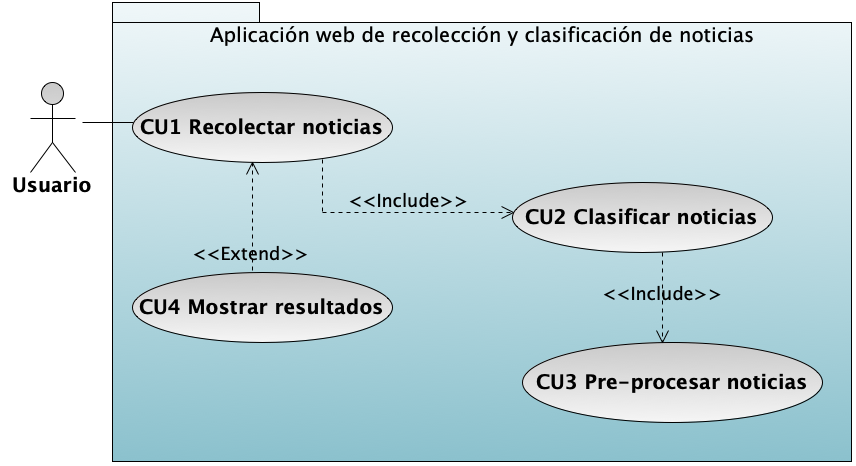
\includegraphics[scale=.4]{imagenes/Diagramas/CasosDeuso/CasosDeuso}
  \caption{Diagrama de casos de uso}
  \label{fig:DCU}
\end{figure}

\newpage


  \newpage
  \Tlabel{CU1}\Tsubsection{CU1 Recolectar noticias}

%================================Intriodcucción==================================%
%----------------------Resumen-----------------------------------%
\begin{large}
	\textbf{Resumen}\\
\end{large}

Brinda al usuario un punto de acceso para elegir una sección; las clasificaciones son, \textbf{Ciencia y tecnología}, \textbf{Política}, \textbf{Deportes}, \textbf{Economía} y  \textbf{Cultura}, posteriormente se recolectan noticias de la web, tomando como punto de partida los sitios establecidos previamente. De cada sitio se recolectan las noticias publicadas; de cada artículo se obtiene \textbf{Fecha de publicación}, \textbf{Título}, \textbf{Contenido}, \textbf{URL de la noticia}, y de contar con ello el \textbf{Resumen}.\\

\begin{large}
	\textbf{Descripción}\\
\end{large} 

%=====================================Tabla 1====================================%


\begin{tabular}{|l|l|}
%-----------------------Ecanbezado-----------------------------------%
	\hline
	\multicolumn{1}{| >{\columncolor{black}}l|}{ \textcolor{myWhite}{\textbf{Caso de uso: }} }&
	\multicolumn{1}{| >{\columncolor{black}}l|}{ \textcolor{myWhite}{CU1 Recolectar noticias} }\\
	\hline
%-----------------------Actor----------------------------------------%
	\textbf{Actor:} & 	Usuario\\
	\hline

%-----------------------Propósito------------------------------------%

	\textbf{Propósito:} & Brindar una herramienta de recolección de noticias\\
	& de Internet(Crawler) \\
	\hline

%----------------------Entradas--------------------------------------%

	\textbf{Entradas:} & URL de las paginas por consultar\\
	\hline

%-----------------------Salidas--------------------------------------%

	\textbf{Salidas:} & \Tref{MSG1}{MSG1 Tiempo de recolección excedido}\\
	\hline

%-----------------------Precondiciones-------------------------------%

	\textbf{Precondición:} & Tener un punto de conexión a Internet\\
	\hline
%-----------------------Postcondiciones------------------------------%

	\textbf{Postcondiciones:} &$\bullet$  El usuario tendrá la facultad\\
	&\ \  de visualizar las noticias clasificadas\\
	&$\bullet$ El usuario podrá cambiar el periodo de búsqueda\\
	\hline

	%-----------------------Reglas de negocio----------------------------%

	\textbf{Reglas de negocio:} &$\bullet$ \RNref{RN1}{Número de palabras}\\
	&$\bullet$ \RNref{RN3}{Listado de fuentes noticiosas}\\
	&$\bullet$ \RNref{RN5}{Orden de publicación}\\
	&$\bullet$ \RNref{RN6}{Periodo de recolección}\\
	&$\bullet$ \RNref{RN7}{Campos recolectados de noticia}\\
	&$\bullet$ \RNref{RN8}{Periodo de actualización}\\
	\hline

%---------------------------Errores----------------------------------%

%------Error 1----------%
	\textbf{Errores:} & $\bullet$ \TError{CU1}{Uno} Cuando el tiempo de \\
	&\ \ recolección se ha excedido se muestra el mensaje\\
	&\ \  \Tref{MSG1}{MSG1 Tiempo de recolección excedido}\\
	\hline

\end{tabular}

\ \\\\

%============================Trayectorias========================================%

%-----------------------Trayectoria Principal-----------------------%


\begin{large}
	\textbf{Trayectoria principal}\\
\end{large}	

\begin{enumerate}[1.]

	
	\item \actor Selecciona una opción de la pantalla \Tref{UI1}{UI1 Inicio}; \textbf{Política}, \textbf{Economía}, \textbf{Deportes}, \textbf{Ciencia y tecnología} o \textbf{Cultura}. 

	\item \sistema Verifica que no existan noticias recolectadas previamente. \TAref{CU1}{A}

	\item \sistema \label{CU1:Recolectar}Muestra la pantalla \Tref{UI2}{Pantalla UI2 Espera de proceso}. 

	\item \sistema Por cada sitio se extraen las noticias con base en la regla de negocio {RN3}{Listado de fuentes noticiosas}, \RNref{RN6}{Periodo de recolección} y \RNref{RN7}{Campos recolectados de noticia.} \TAref{CU1}{D}

	\item \label{CU1:BuscarN}\sistema Incluye el caso de uso \textbf{CU2 Clasificar noticias}.

	\item \sistema \label{CU1:NoticiasR} Se obtienen las noticias clasificadas de la sección seleccionada por el usuario, de acuerdo a la regla de negocio \RNref{RN5}{Orden de publicación.}

	\item \sistema Muestra la pantalla \Tref{UI3}{Pantalla UI3 Proceso concluido}.

	\item \finCU	

\end{enumerate}







%-------------------------trayectoria Alternativa A-----------------%
\begin{large}
	\Talterna{CU1}{A}\\
\end{large}	
\textbf{Condición:} \textit{Existen noticias recolectadas}

\begin{enumerate}[{A-}1.]

	\item \sistema Verifica que la última recolección de noticias no exceda el periodo establecido, con base \RNref{RN8}{Periodo de actualización}.

	\item \actor Continua en el paso \ref{CU1:NoticiasR} de la trayectoria principal.

	\item \finTA

\end{enumerate}

%-------------------------trayectoria Alternativa B-----------------%
\begin{large}
	\Talterna{CU1}{B}\\
\end{large}	
\textbf{Condición:} \textit{La última recolección de noticias excede el periodo establecido}

\begin{enumerate}[{B-}1.]

	\item \actor Continua en el paso \ref{CU1:Recolectar} de la trayectoria principal.

	\item \finTA

\end{enumerate}


%================================Puntos de extención=============================%


\begin{large}
	\textbf{Puntos de extensión}\\
\end{large}	

%--------------------Puntos de extención 1------------------------%
\textbf{Causa de la extensión:} El usuario desea consultar las noticias clasificadas.\\
\textbf{Región de la trayectoria:} Proviene del paso \ref{CU1:NoticiasR} de la trayectoria principal.\\
\textbf{Extiende a :} \Tref{CU4}{CU4 Mostrar resultados}\\\\



  \newpage
  \Tlabel{CU2}\Tsubsection{CU2 Clasificar noticias}

%================================Intriodcucción==================================%
%----------------------Resumen-----------------------------------%
\begin{large}
	\textbf{Resumen}\\
\end{large}

Brinda al sistema una herramienta que permite realizar la clasificación de las noticias recolectadas, en las secciones \textbf{Ciencia y tecnología}, \textbf{Política}, \textbf{Deportes}, \textbf{Economía} y  \textbf{Cultura}, utilizando como modelo clasificador el algoritmo \textbf{Máquina de Soporte Vectorial}. Además el conjunto de noticias clasificadas es almacenado en un archivo por cada sección. Cabe señlar que las descargas se hacen en un periodo establecido.\\


\begin{large}
	\textbf{Descripción}\\
\end{large} 

%=====================================Tabla 1====================================%


\begin{tabular}{|l|l|}
%-----------------------Encabezado-----------------------------------%
	\hline
	\multicolumn{1}{| >{\columncolor{black}}l|}{ \textcolor{myWhite}{\textbf{Caso de uso: }} }&
	\multicolumn{1}{| >{\columncolor{black}}l|}{ \textcolor{myWhite}{CU1 Recolectar noticias} }\\
	\hline
%-----------------------Actor----------------------------------------%
	\textbf{Actor:} & 	Usuario\\
	\hline

%-----------------------Propósito------------------------------------%

	\textbf{Propósito:} & Clasificar las noticias recolectadas\\
	\hline

%----------------------Entradas--------------------------------------%

	\textbf{Entradas:} &  $\bullet$ Noticias recolectadas\\
	& $\bullet$ Modelo clasificador\\
	\hline

%-----------------------Salidas--------------------------------------%

	\textbf{Salidas:} & Los archivos de cada sección los cuales contienen\\	
	& el conjunto de noticias correspondientes\\
	\hline

%-----------------------Precondiciones-------------------------------%

	\textbf{Precondiciones:} & Debe existir al menos una noticia recolectada\\
	\hline
%-----------------------Postcondiciones------------------------------%

	\textbf{Postcondiciones:} & Las noticias clasificadas podrán ser obtenidas \\
	& por el sistema\\
	\hline

	%-----------------------Reglas de negocio----------------------------%

	\textbf{Reglas de negocio:} & Ninguna\\
	\hline

%---------------------------Errores----------------------------------%

%------Error 1----------%
	\textbf{Errores:} & Ninguno\\

	\hline

\end{tabular}
\ \\\\


%-----------------------Trayectoria Principal-----------------------%


\begin{large}
	\textbf{Trayectoria principal}\\
\end{large}	

\begin{enumerate}[1.]

		
	\item \sistema Obtiene las noticias recolectadas.

	\item \sistema Incluye el caso de uso \textbf{CU3 Pre-procesar noticias}.

	\item \sistema \label{CU2:vocabulario}Obtiene el vocabulario definido, para el modelo clasificador.

	\item \sistema Generá un vector de características por cada noticia, con base al vocabulario del paso \ref{CU2:vocabulario}.

	\item \sistema Obtiene el modelo clasificador.

	\item \sistema Clasifica las noticias recolectadas.

	\item \sistema Almacena las noticias clasificadas por sección.
	
	\item \finCU	

\end{enumerate}

  \Tlabel{CU3}\Tsubsection{CU3 Pre-procesar noticias}

%================================Intriodcucción==================================%
%----------------------Resumen-----------------------------------%
\begin{large}
	\textbf{Resumen}\\
\end{large}

Realiza dos tareas fundamentales, previas al proceso de clasificación las cuales son: \textbf{Tokenizar}. Este proceso consiste en dividir el texto en sus elementos mínimos llamados tokens, donde se separan palabras, signos de puntuación, llaves y números mediante un espacio; \textbf{Lematizar}. Esta tarea reduce cada palabra en su lema, con el objetivo de simplificar el vocabulario de un texto. Es importante mencionar que, de cada artículo se extrae la \textbf{URL}, \textbf{Título}, \textbf{Fecha} \textbf{Redacción de la noticia}, y de existir un \textbf{Resumen}. Sin embargo para el proceso de clasificación solo se utiliza la redacción de la noticia.\\ 


\begin{large}
	\textbf{Descripción}\\
\end{large} 

%=====================================Tabla 1====================================%


\begin{tabular}{|l|l|}
%-----------------------Ecanbezado-----------------------------------%
	\hline
	\multicolumn{1}{| >{\columncolor{black}}l|}{ \textcolor{myWhite}{\textbf{Caso de uso: }} }&
	\multicolumn{1}{| >{\columncolor{black}}l|}{ \textcolor{myWhite}{CU1 Recolectar noticias} }\\
	\hline
%-----------------------Actor----------------------------------------%
	\textbf{Actor:} & 	Usuario\\
	\hline

%-----------------------Propósito------------------------------------%

	\textbf{Propósito:} & Preparar el contenido de las noticias para el proceso\\
	&de extracción de características\\
	\hline

%----------------------Entradas--------------------------------------%

	\textbf{Entradas:} & Contenido de los artículos recolectados\\
	\hline

%-----------------------Salidas--------------------------------------%

	\textbf{Salidas:} & Contenido procesado de los artículos \\	
	\hline

%-----------------------Precondiciones-------------------------------%

	\textbf{Precondición:} & Vocabulario en español para el proceso\\
	& de lematización\\
	\hline
%-----------------------Postcondiciones------------------------------%

	\textbf{Postcondiciones:} & Se podrá generar el vector de características\\
	&de cada noticia\\
	\hline

	%-----------------------Reglas de negocio----------------------------%

	\textbf{Reglas de negocio:} & Ninguna \\
	\hline

%---------------------------Errores----------------------------------%

%------Error 1----------%
	\textbf{Errores:} & Ninguno \\

	\hline

\end{tabular}
\ \\\\


%-----------------------Trayectoria Principal-----------------------%


\begin{large}
	\textbf{Trayectoria principal}\\
\end{large}	

\begin{enumerate}[1.]

	
	\item \sistema Obtiene la redacción de las noticias.

	\item \sistema Obtiene el vocabulario en español.

	\item \sistema Realiza el proceso de tokenización.

	\item \sistema Realiza el proceso de lematización.
	
	\item \finCU	

\end{enumerate}

  
  \newpage
  \Tlabel{CU4}\Tsubsection{CU4 Mostrar resultados}

%================================Intriodcucción==================================%
%----------------------Resumen-----------------------------------%

\begin{large}
	\textbf{Resumen}\\
\end{large}

Permite al actor visualizar las noticias correspondiente a la sección elegida, ya sea \textbf{Política}, \textbf{Deportes}, \textbf{Ciencia y tecnología}, \textbf{Economía} o \textbf{Cultura}. Cada artículo contiene el \textbf{Título}, \textbf{Autor}, la \textbf{Fecha de publicación}, \textbf{URL} el cual direcciona a la página fuente que ha proporcionado la noticias y de contar con ello un \textbf{Resumen de la noticia}. Además se permite filtrar las noticias en un periodo de al menos tres días. Cabe destacar que las noticias mostradas por defecto, corresponden a la fecha actual.\\

\begin{large}
	\textbf{Descripción}\\
\end{large}



%=====================================Tabla 1====================================%
\begin{table}[H]
	\centering
	\begin{tabular}{|l|l|}

	%-----------------------Ecanbezado-----------------------------------%
		\hline
		\multicolumn{1}{| >{\columncolor{black}}l|}{ \textcolor{myWhite}{\textbf{Caso de uso: }} }&
		\multicolumn{1}{| >{\columncolor{black}}l|}{ \textcolor{myWhite}{CU4 Mostrar resultados} }\\
		\hline
	%-----------------------Actor----------------------------------------%
		\textbf{Actor:} & 	Usuario	\\
		\hline
	%-----------------------Propósito------------------------------------%
		\textbf{Propósito:} & Brindar una herramienta que permita consultar las\\
		&noticias clasificadas y filtradas por su fecha de publicación\\
		\hline

	%----------------------Entradas--------------------------------------%
		\textbf{Entradas:} &Periodo de búsqueda\\
		\hline

	%-----------------------Salidas--------------------------------------%
		\textbf{Salidas:}&$\bullet$ \Tref{MSG2}{MSG2 Petición vacía}\\
		&$\bullet$ Noticias clasificadas; de cada una se muestra:\\
		&\ \ $\circ$ \textbf{Título}\\
		&\ \ $\circ$ \textbf{URL al artículo}\\
		&\ \ $\circ$ \textbf{Fecha de publicación}\\
		&\ \ $\circ$ \textbf{Autor}\\
		&\ \ $\circ$ \textbf{Resumen}\\
		\hline

	%-----------------------Precondiciones-------------------------------%

		\textbf{Precondición:} & Las noticias clasificadas deben estar \\
		&almacenadas por sección\\
		\hline

	%-----------------------Postcondiciones------------------------------%

	%---------Post 1----------%
		\textbf{Postcondiciones:}& Ninguna\\
		\hline

	%-----------------------Reglas de negocio----------------------------%
		\textbf{Reglas de negocio:}& \RNref{RN5}{Orden de publicación}\\
		\hline
	%---------------------------Errores----------------------------------%

	%------Error 1----------%
		\textbf{Errores:} &\TError{CU4}{Uno} Cuando no se ha encontrado noticias en el\\
		&\ \ día seleccionado se muestra el mensaje \Tref{MSG2}{MSG2}\\
		&\ \ \Tref{MSG2}{Petición vacía}\\
		\hline

	\end{tabular}

	%\caption{ Tabla de descripción de CU4 }
\end{table}
%============================Trayectorias========================================%

%-----------------------Trayectoria Principal-----------------------%

\begin{large}
	\textbf{Trayectoria principal}\\
\end{large}	

\begin{enumerate}[1.]

	\item \actor Presiona el botón \textbf{Continuar} de la pantalla \Tref{UI3}{Pantalla UI3 Proceso concluido}. \TAref{CU1}{A}

	\item \sistema Obtiene la fecha actual.

	\item \sistema Muestra al menos 5 noticias, de acuerdo a la regla de negocio \RNref{RN5}{Orden de publicación} de la sección previamente elegida (filtro de sección) y del día actual (filtro de fecha), como se visualiza en la pantalla \Tref{UI4}{UI4 Resultados de consulta}.

	\item \actor \label{CU4:Consulta}Consulta la noticia.\TAref{CU4}{B}

	\item \finCU	
\end{enumerate}


%-------------------------trayectoria Alternativa A-----------------%
\begin{large}
	\Talterna{CU4}{A}\\
\end{large}	
\textbf{Condición:} \textit{El usuario ha presionado el botón cancelar}

\begin{enumerate}[{A-}1.]

	\item \actor Presiona el botón \textbf{Cancelar} de la pantalla \Tref{UI3}{Pantalla UI3 Proceso concluido}.

	\item \sistema Muestra la pantalla \Tref{UI1}{UI1 Inicio}.

	\item \finTA

\end{enumerate}


%-------------------------trayectoria Alternativa B-----------------%
\begin{large}
	\Talterna{CU4}{B}\\
\end{large}	
\textbf{Condición:} \textit{El usuario ha cambiado el periodo establecido}

\begin{enumerate}[{B-}1.]

	\item \actor \label{CU4:Dia}Presiona un botón del menú \textbf{Cambio de periodo} de la pantalla \Tref{UI4}{UI4 Resultados de consulta}.

	\item \sistema Verifica que exista al menos 1 noticia en el periodo establecido. \TAref{CU4}{C}

	\item \sistema Muestra noticias de acuerdo a la regla de negocio \RNref{RN5}{Orden de publicación} de la sección previamente elegida (filtro de sección) y del día seleccionado en el paso \ref{CU4:Dia} (filtro de fecha), como se visualiza en la pantalla \Tref{UI5}{UI5 Cambio de periodo}.

	\item \sistema Continua en el paso \ref{CU4:Consulta} de la trayectoria principal.

	\item \finTA

\end{enumerate}


%-------------------------trayectoria Alternativa C-----------------%
\begin{large}
	\Talterna{CU4}{C}\\
\end{large}	
\textbf{Condición:} \textit{No se ha encontrado noticias del día seleccionado \TEref{CU4}{Uno}}

\begin{enumerate}[{C-}1.]

	\item \sistema Muestra el mensaje \Tref{MSG2}{MSG2 Petición vacía}, en la pantalla \Tref{UI4}{UI4 Resultados de consulta}.

	\item \sistema Continua en el paso \ref{CU4:Consulta} de la trayectoria principal.

	\item \finTA

\end{enumerate}


  \newpage

%------------------------Mensajes----------------------------------%

\section{Mensajes}
  
  %------------------MSG1-----------------------%
     \Mline{MSG1}{Tiempo de recolección excedido}
    \begin{itemize}
      \item \textbf{Tipo:} Error. 
      \item \textbf{Objetivo:}  Dar a conocer que se ha excedido el tiempo de recolección de noticias de los sitios web definidos.
      \item \textbf{Redacción:} Se ha agotado el tiempo de espera, no se han encontrado noticias. Intentar más tarde.
      \item \textbf{Referenciado por:} \Tref{CU1}{CU1 Recolectar noticias}\\
    \end{itemize}

  %------------------MSG2-----------------------%
   \Mline{MSG2}{Petición vacía}
  \begin{itemize}
    \item \textbf{Tipo:} Error. 
    \item \textbf{Objetivo:}  Informar al usuario que no se ha encontrado resultados en el día seleccionado.
    \item \textbf{Redacción:}  No se ha encontrado noticias en el día seleccionado.

    \item \textbf{Referenciado por:} \Tref{CU4}{CU4 Mostrar resultados}\\
  \end{itemize}

  %------------------MSG3-----------------------%
   \Mline{MSG3}{Fallo en la recolección}
  \begin{itemize}
    \item \textbf{Tipo:} Error. 
    \item \textbf{Objetivo:}  Informar al usuario que las ligas registradas en el diccionario de \textbf{URLs} no permiten extraer información.
    \item \textbf{Redacción:} No se puede extraer noticias de los sitios registrados en este portal web.
    \item \textbf{Referenciado por:} \Tref{CU1}{CU1 Recolectar noticias}\\
  \end{itemize}

  %------------------MSG4-----------------------%
%   \Mline{MSG4}{Fallo al ingresar a sitio web}
%  \begin{itemize}
%    \item \textbf{Tipo:} Error. 
%    \item \textbf{Objetivo:} Informar al usuario sobre el fallo ocurrido en la conexión del portal web seleccionado.
%    \item \textbf{Redacción:} Ha ocurrido un fallo en la conexión con el sitio seleccionado, intente mas tarde.
%    \item \textbf{Referenciado por:} \Tref{CU7}{CU7 Ingresar a sitio web}\\
%  \end{itemize}

\newpage

  %--------------------------Descripción de pantallas ------------------%
\section{Pantallas}

\Tsubsection{UI1 Página de inicio} 
%------------------------------------Objetivo----------------------------------%
\begin{large}
  \textbf{Objetivo}\\
\end{large}


Permite al usuario seleccionar la sección a consultar.\\

%------------------------------------Descripción---------------------------------%
\begin{large}
  \textbf{Descripción}\\
\end{large}

La Pantalla \ref{fig:UI1} muestra un menú con las secciones definidas para el sistema las cuales son: \textbf{Política}, \textbf{Deportes}, \textbf{Ciencia y tecnología}, \textbf{Economía} y \textbf{Cultura}. En ella se puede navegar para acceder a la consulta de las noticias recolectadas y clasificadas de alguna sección.\\

%-----------------------------------Salidas------------------------------------%
\begin{large}
  \textbf{Salidas}
\end{large}

\begin{itemize}

  \item \Tref{MSG2}{MSG2 Tiempo de recolección excedido}

\end{itemize}

%------------------------------------Comandos----------------------------------%

\textbf{Comandos}

\begin{enumerate}

  \item \textbf{Inicio}: Direcciona a la pantalla descrita en esta sección
  \item \textbf{Política}: Permite realizar una consulta en la sección Política
  \item \textbf{Deportes}: Permite realizar una consulta en la sección Deportes
  \item \textbf{Ciencia y tecnología}: Permite realizar una consulta en la sección Ciencia
  \item \textbf{Economía}: Permite realizar una consulta en la sección Economía
  \item \textbf{Cultura}: Permite realizar una consulta en la sección Cultura

\end{enumerate}

%------------------------------------Referencia----------------------------------%
\begin{large}
  \textbf{Referenciado por}
\end{large}

\begin{itemize}

  \item \Tref{CU1}{CU1 Recolectar noticias}
  \item \Tref{CU4}{CU4 Mostrar resultados}

\end{itemize}  

%----------------------------------------Pantalla--------------------------------%

\begin{figure}\Tlabel{UI1}
  \centering
	
\includegraphics[scale=.35]{imagenes/Pantallas/UI1}
  \caption{Pantalla UI1 Inicio}
  \label{fig:UI1}
\end{figure}



\Tsubsection{UI2 Recolección y clasificación} 
%------------------------------------Objetivo----------------------------------%
\begin{large}
  \textbf{Objetivo}\\
\end{large}


Informar al usuario que la recolección y clasificación de noticias se está llevando acabo.\\

%------------------------------------Descripción---------------------------------%
\begin{large}
  \textbf{Descripción}\\
\end{large}

La Pantalla \ref{fig:UI2} muestra un mensaje flotante con la siguiente redacción: \textbf{En proceso de recolección y clasificación}, para informar al usuario que la consulta realizada está en proceso.\\

%-----------------------------------Salidas------------------------------------%
\begin{large}
  \textbf{Salidas}
\end{large}

\begin{itemize}

  \item Ninguno

\end{itemize}

%------------------------------------Comandos----------------------------------%


%------------------------------------Referencia----------------------------------%
\begin{large}
  \textbf{Referenciado por}
\end{large}

\begin{itemize}

  \item \Tref{CU1}{CU1 Recolectar noticias}

\end{itemize}  

%----------------------------------------Pantalla--------------------------------%


\begin{figure}\Tlabel{UI2}
  \centering 
	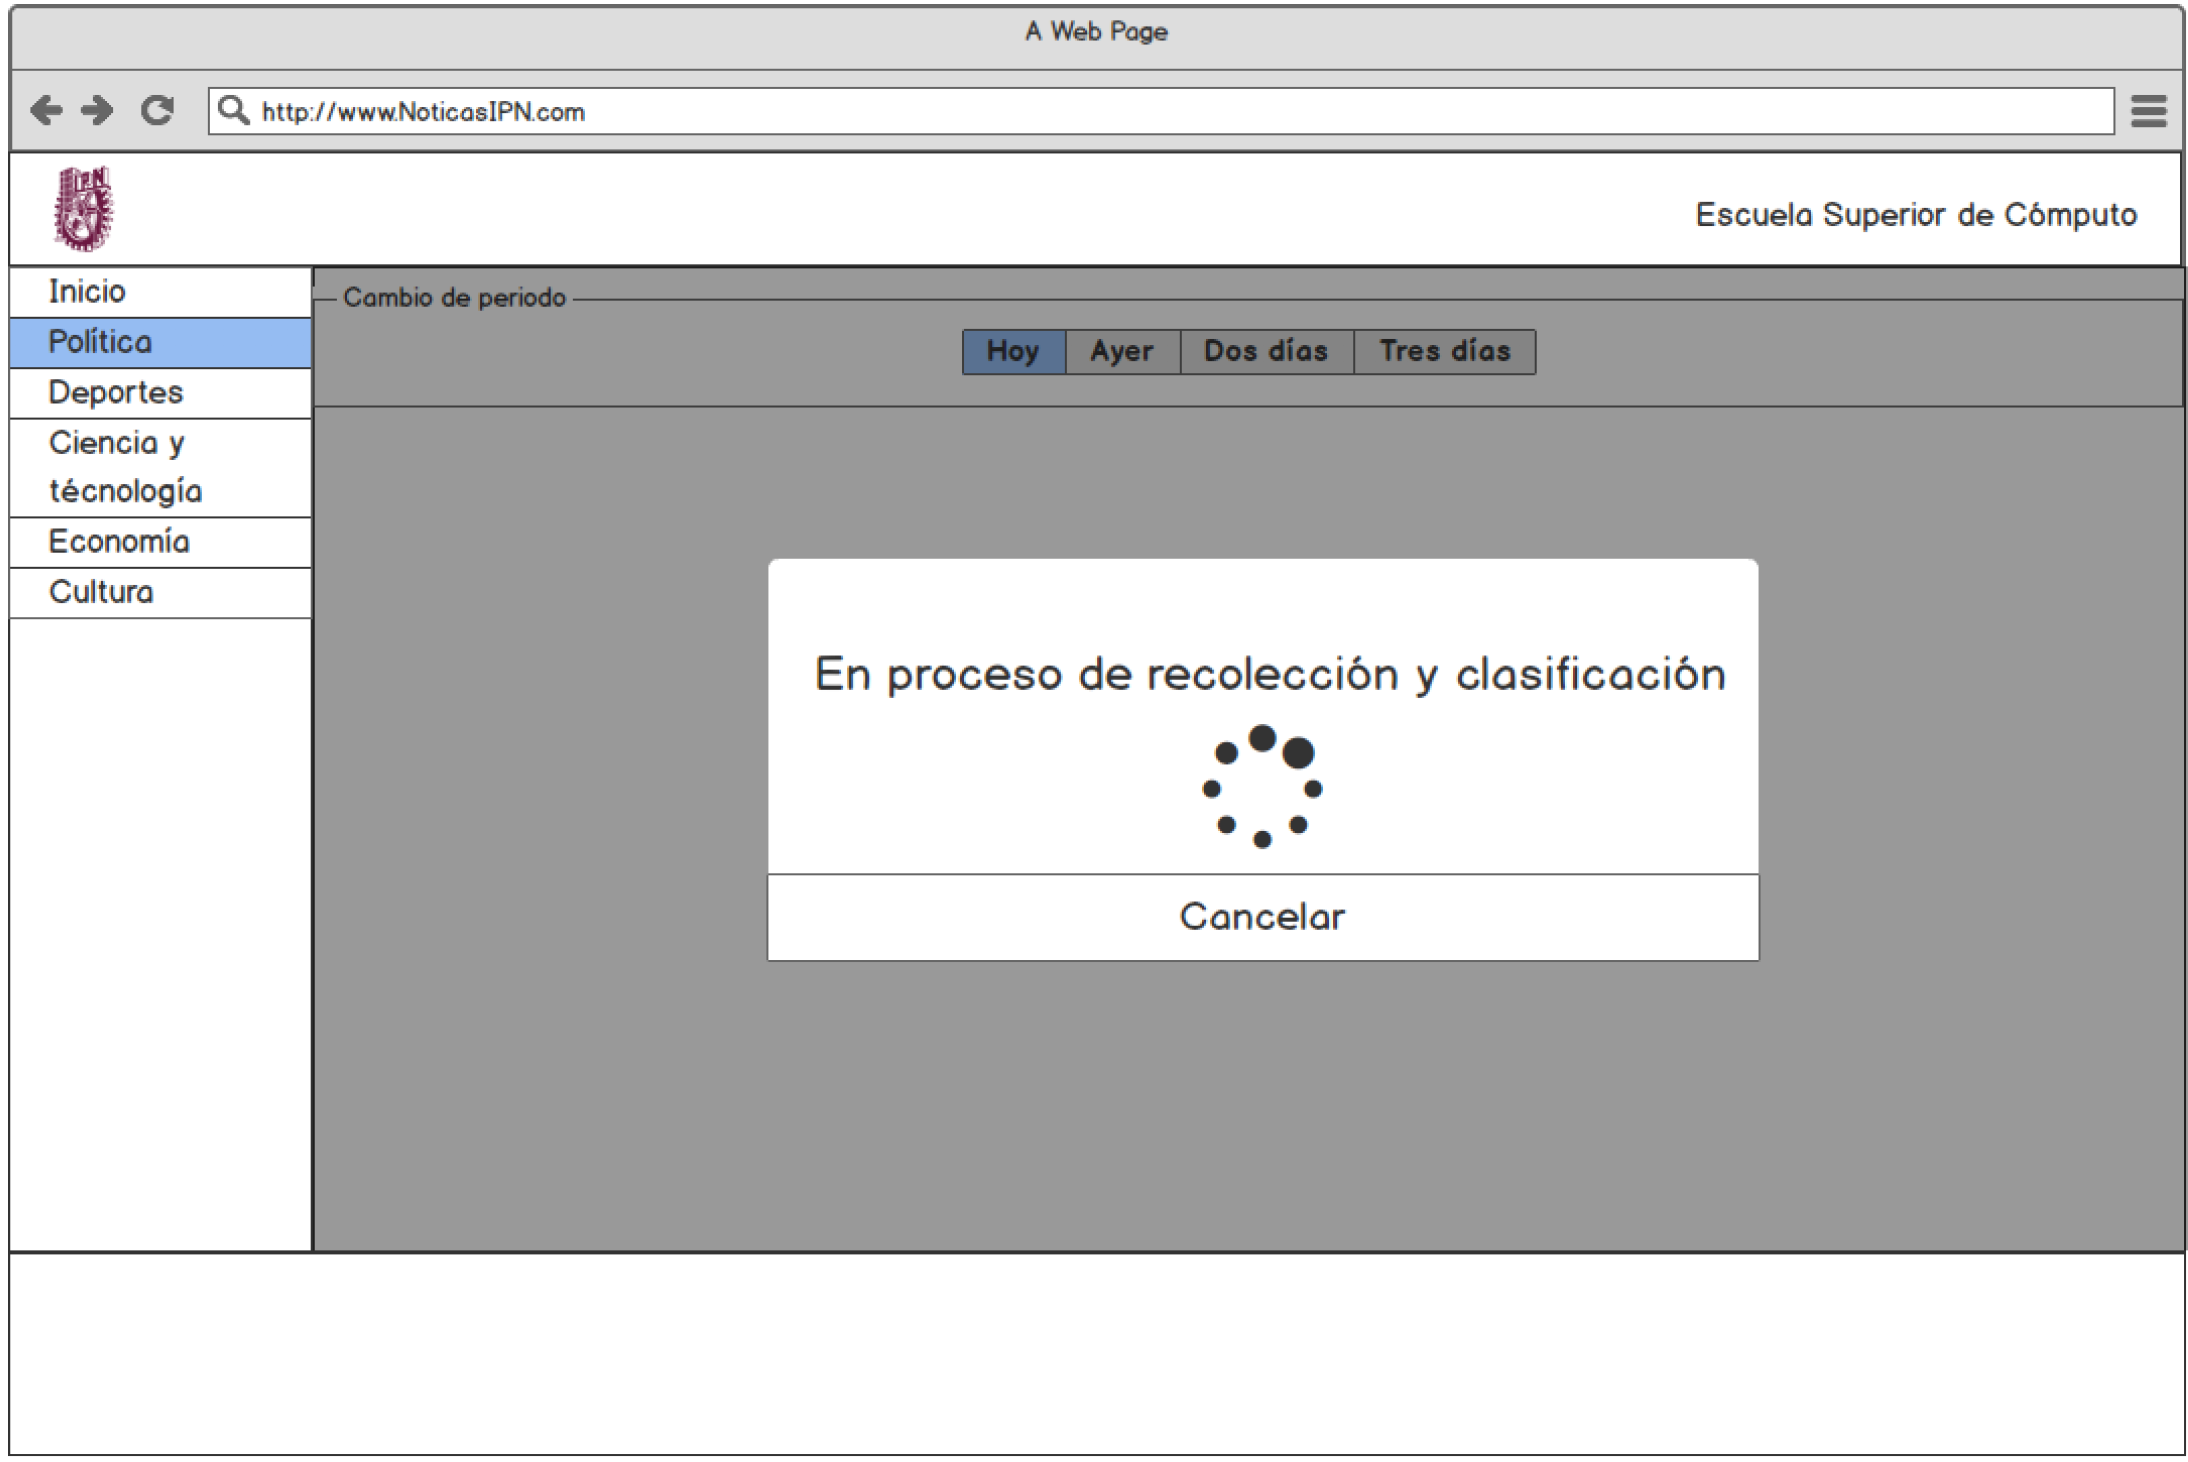
\includegraphics[scale=.32]{imagenes/Pantallas/UI2}
  \caption{Pantalla UI2 Espera de proceso}
  \label{fig:UI2}
\end{figure}

\Tsubsection{UI3 Proceso concluido} 
%------------------------------------Objetivo----------------------------------%
\begin{large}
  \textbf{Objetivo}\\
\end{large}


Informal al usuario que la recolección y clasificación ha concluido y brinda un punto de acceso para visualizar los resultados de la consulta.\\

%------------------------------------Descripción---------------------------------%
\begin{large}
  \textbf{Descripción}\\
\end{large}

La Pantalla \ref{fig:UI3} muestra un mensaje flotante con la siguiente redacción: \textbf{Noticias listas para ser mostradas}, el cual informa al usuario que el proceso de recolección y clasificación ha concluido, \textit{i.e} ya se pueden mostrar las noticias clasificadas de la sección elegida. En la parte inferior se muestra el botón \textbf{Cancelar} y \textbf{Continuar}.  \\

%-----------------------------------Salidas------------------------------------%
\begin{large}
  \textbf{Salidas}
\end{large}

\begin{itemize}

  \item Ninguno

\end{itemize}

%------------------------------------Comandos----------------------------------%

\textbf{Comandos}

\begin{enumerate}

  \item \textbf{Cancelar}: Detiene el proceso de recolección y clasificación, re-direcciona a la pantalla \Tref{UI1}{UI1 Inicio}.
  \item \textbf{Continuar}: Permite avanzar para visualizar las noticias clasificadas de la sección elegida en la pantalla \Tref{UI4}{UI4 Resultados de consulta}

\end{enumerate}

%------------------------------------Referencia----------------------------------%
\begin{large}
  \textbf{Referenciado por}
\end{large}

\begin{itemize}

  \item \Tref{CU1}{CU1 Recolectar noticias}
  \item \Tref{CU4}{CU4 Mostrar resultados}

\end{itemize}  

%----------------------------------------Pantalla--------------------------------%

\begin{figure}\Tlabel{UI3}
  \centering
	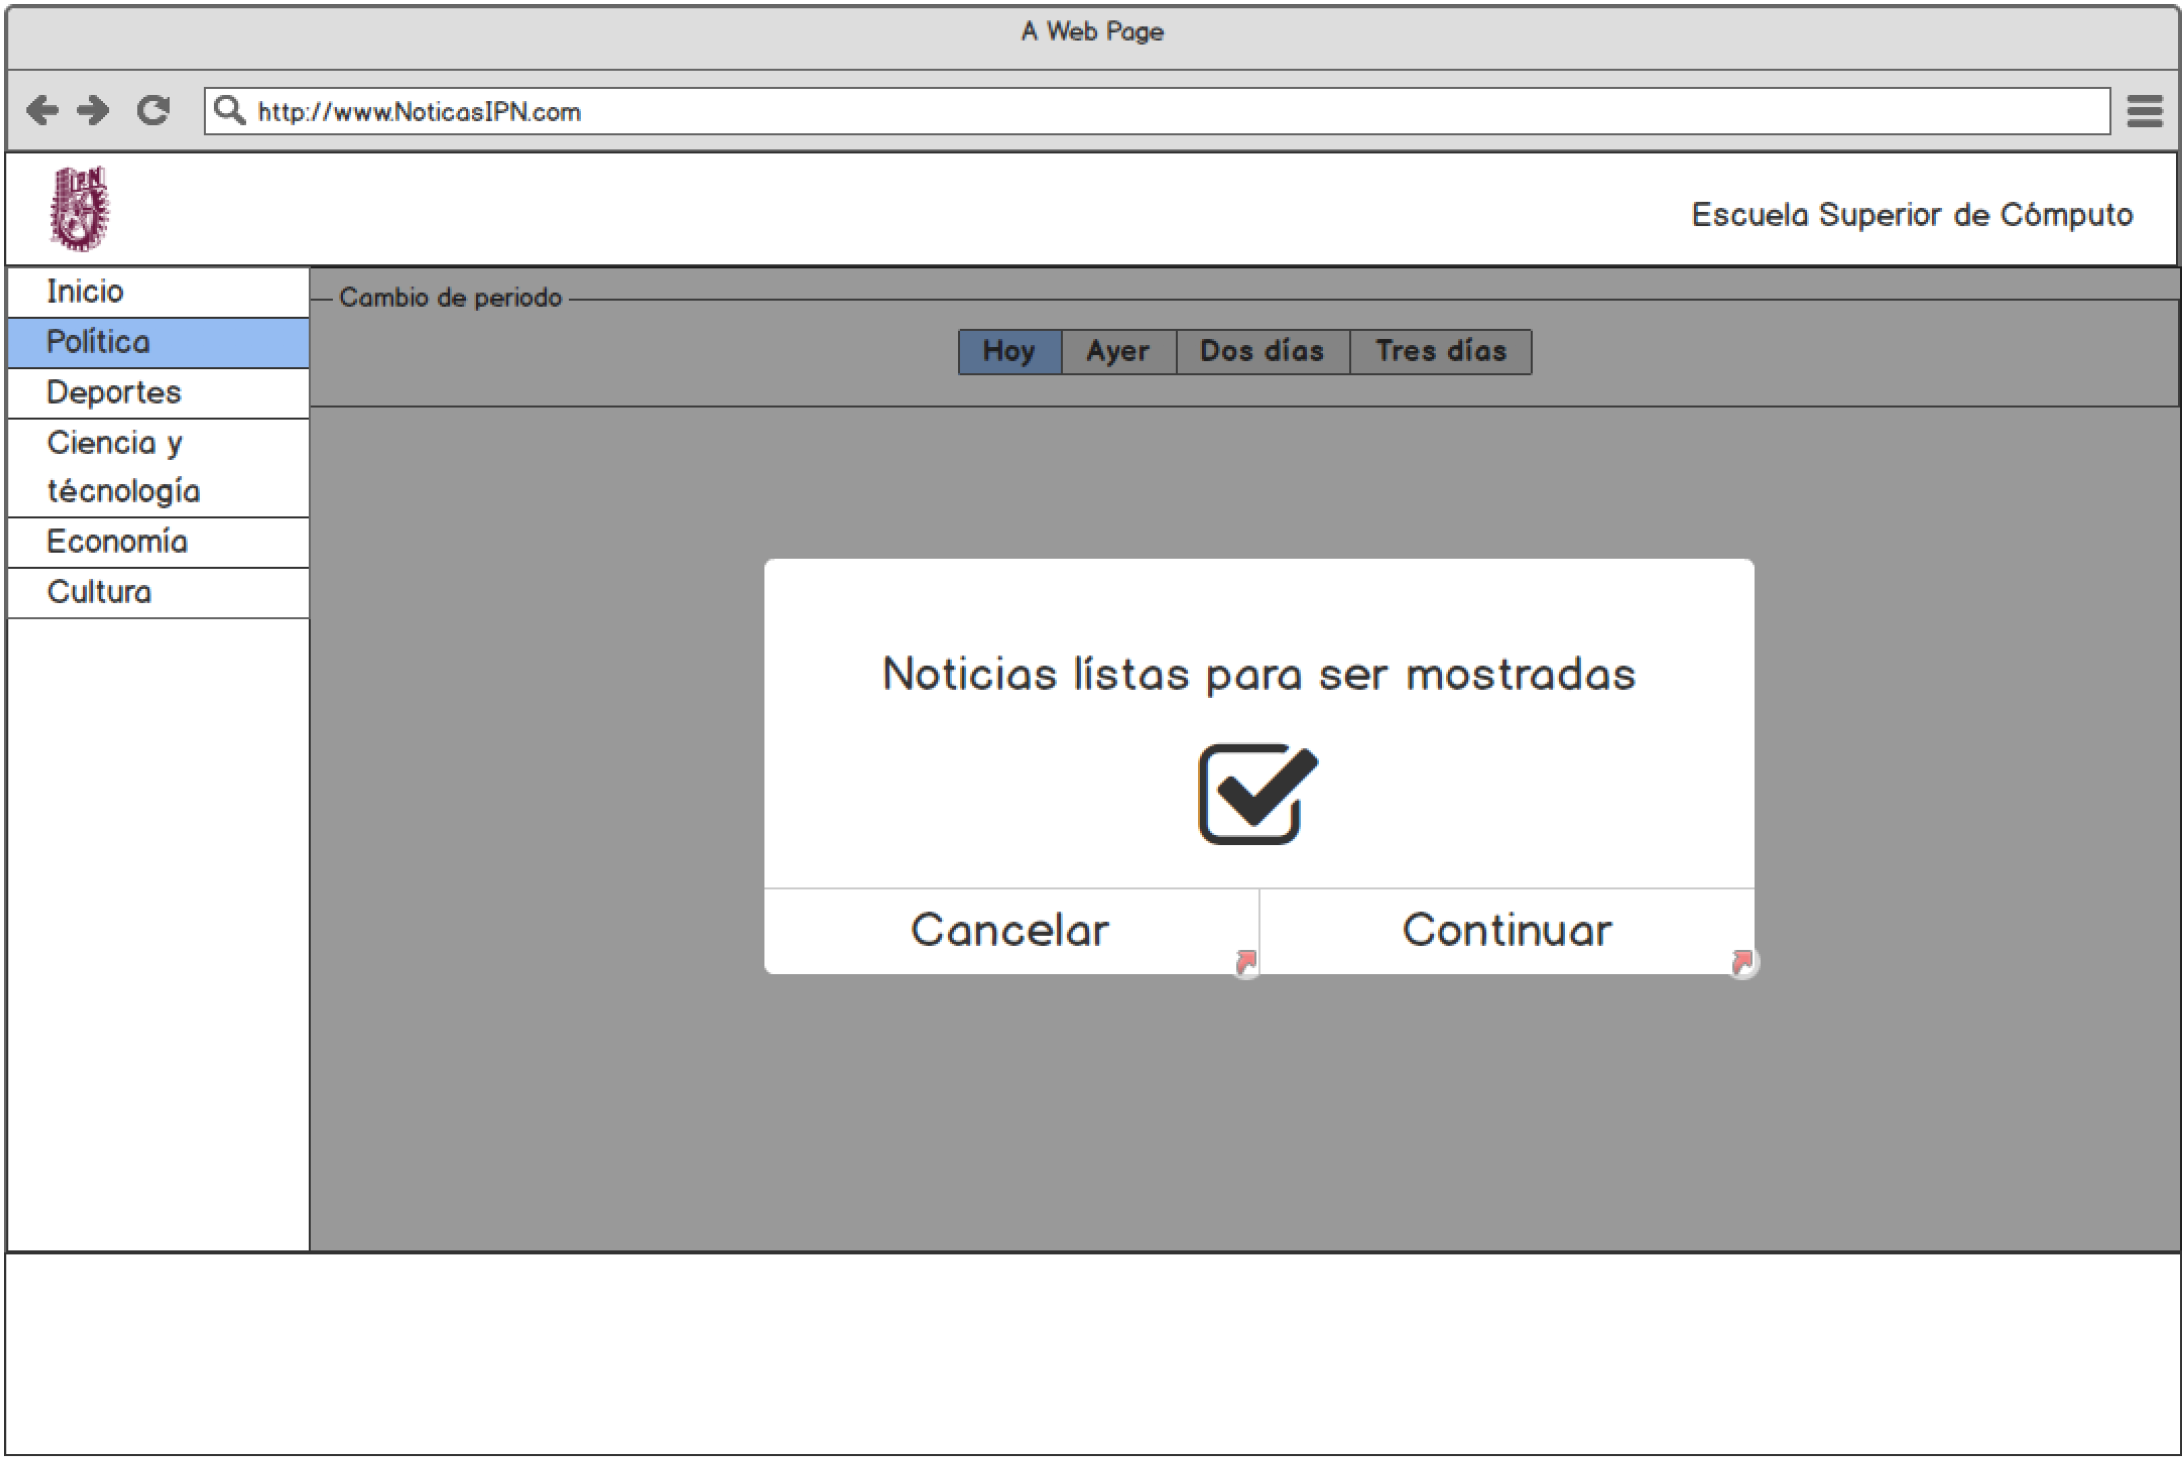
\includegraphics[scale=.35]{imagenes/Pantallas/UI3}
  \caption{Pantalla UI3 Proceso concluido}
  \label{fig:UI3}
\end{figure}

\Tsubsection{UI4 Resultados de consulta} 
%------------------------------------Objetivo----------------------------------%
\begin{large}
  \textbf{Objetivo}\\
\end{large}


Permite consultar las noticias clasificadas en la sección previamente elegida. Además brinda una forma de cambiar el periodo de búsqueda y permite entrar al sitio de origen de los artículos mostrados.\\

%------------------------------------Descripción---------------------------------%
\begin{large}
  \textbf{Descripción}\\
\end{large}

La Pantalla \ref{fig:UI4} muestra una sección con las noticias clasificadas, de cada noticia se muestra:

\begin{itemize}

  \item \textbf{Título}
  \item \textbf{URL al artículo}
  \item \textbf{Fecha de publicación}
  \item \textbf{Resumen}

\end{itemize}

En la parte superior de la pantalla se muestra el menú \textbf{Cambio de periodo} el cual permite cambiar le periodo de consulta de las noticias. Cabe señalar que la primera vez que se ingresa a esta pantalla se muestran los artículos con fecha de publicación del día actual.
La Pantalla \ref{fig:UI5} muestra un ejemplo de consulta en una fecha diferente.



%-----------------------------------Salidas------------------------------------%
\begin{large}
  \textbf{Salidas}
\end{large}

\begin{itemize}

  \item \Tref{MSG2}{MSG2 Petición vacía}

\end{itemize}

%------------------------------------Comandos----------------------------------%

\textbf{Comandos}

\begin{enumerate}

  \item \textbf{Hoy}: Realiza la consulta en la fecha actual
  \item \textbf{Ayer}: Realiza la consulta un día antes de la fecha actual
  \item \textbf{Dos días}: Realiza la consulta dos días antes de la fecha actual
  \item \textbf{Tres días}: Realiza la consulta tres días antes de la fecha actual
  \item \textbf{URL}: La url que muestra la noticia direcciona al sitio web de recolección


\end{enumerate}

%------------------------------------Referencia----------------------------------%
\begin{large}
  \textbf{Referenciado por}
\end{large}

\begin{itemize}

  \item \Tref{CU4}{CU4 Mostrar resultados}

\end{itemize}  

%----------------------------------------Pantalla--------------------------------%


%-----------------------------UI1--------------------------%
\begin{figure}\Tlabel{UI4}
  \centering
  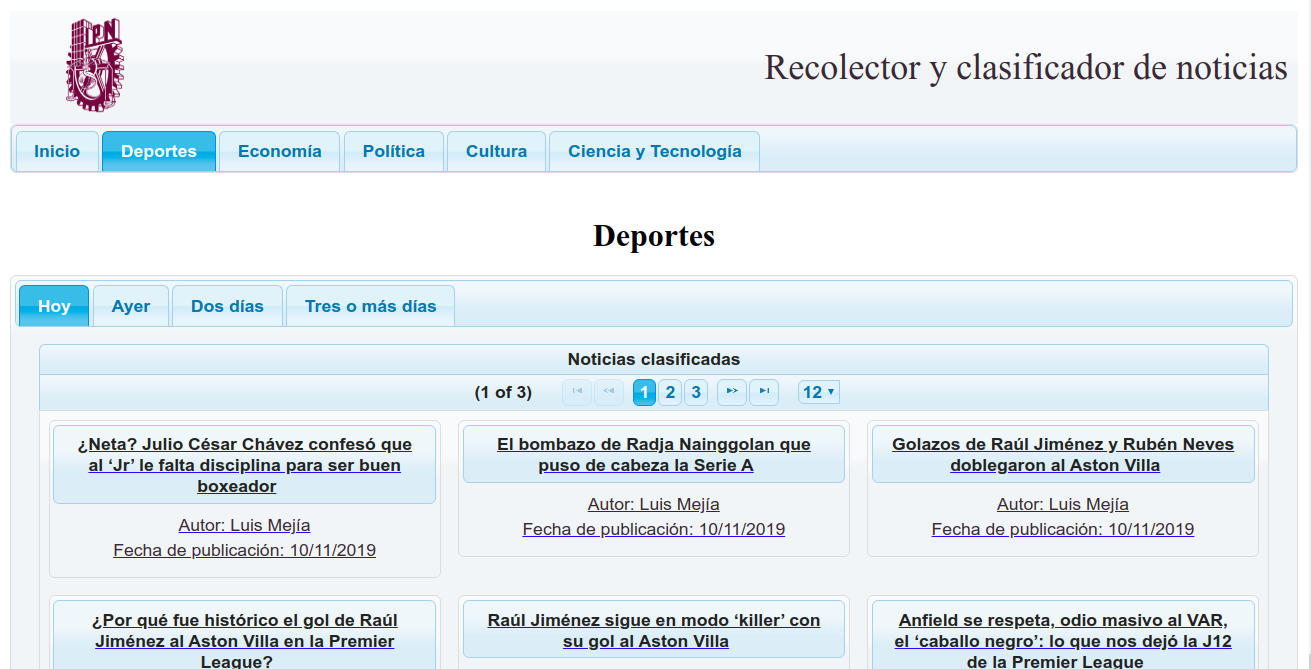
\includegraphics[scale=.32]{imagenes/Pantallas/UI4}
  \caption{Pantalla UI4 Resultados de consulta}
  \label{fig:UI4}
\end{figure}

%-----------------------------UI2--------------------------%
\begin{figure}\Tlabel{UI5}
  \centering
  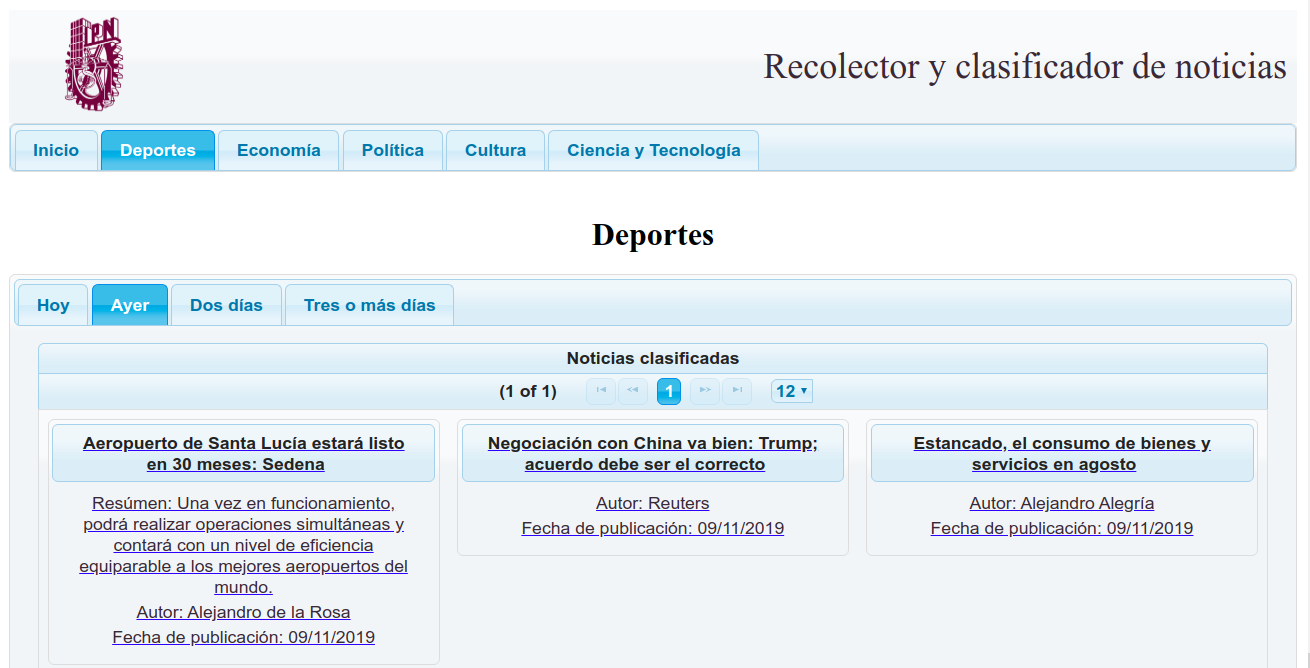
\includegraphics[scale=.32]{imagenes/Pantallas/UI5}
  \caption{Pantalla UI5 Cambio de periodo}
  \label{fig:UI5}
\end{figure}



\newpage


%-------------------------------Diagrama de secuencia

\section{Diagrama de secuencia}




La figura \textbf{\ref{fig:DSE}} muestra el diagrama de secuencia de la aplicación. 

\begin{figure}[H]
  \centering
  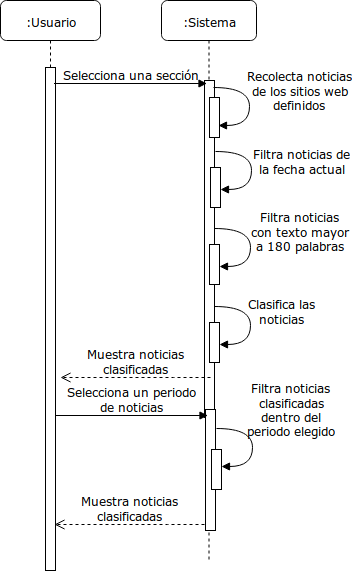
\includegraphics[scale=.75]{imagenes/Diagramas/Secuencia/Diagrama}
  \caption{Diagrama de secuencia}
  \label{fig:DSE}
\end{figure}

\newpage

